\section{Durchführung}
\label{sec:Durchführung}

\subsection{Aufnahme der Kennlinie}

Zur Aufnahme der Kennlinien wird die Schaltung aus Abbildung \ref{fig:aufbau1} verwendet. Der 
Heizstrom im Bereich von $\SI{2.1}{\ampere}$ bis $\SI{2.5}{\ampere}$ wird mit einem
Konstantsspannungsgerät erzeugt. Der Heizstrom $I_\text{F}$ wird an der integierten 
Anzeige abgelesen. Für die Bestimmung der Heizspannung $U_\text{F}$ wird der ebenfalls
integierte Voltmeter verwendet, das aber nur eine grobe Auflösung liefert. Die 
Anodenspannung $U$, die mit einem zweiten Konstantsspannungsgerät erzeugt wird, wird
einem eingebauten Messgerät entnommen. Der Anodenstrom $I$ kann ebenfalls dort
abgelesen werden. Vor das Netzgerät wird ein Widerstand von $\SI{100}{\ohm}$ geschaltet,
sodass durch die abfallende Spannung Rückschlüsse auf den Anodenstrom gezogen werden 
können. Anstatt der Kurve des $x-y$-Schreibers werden Messwerte der Anodenspannung 
und des Anodenstroms für die verschiedenen Heizströme abgelesen. 

\begin{figure}
  \centering
  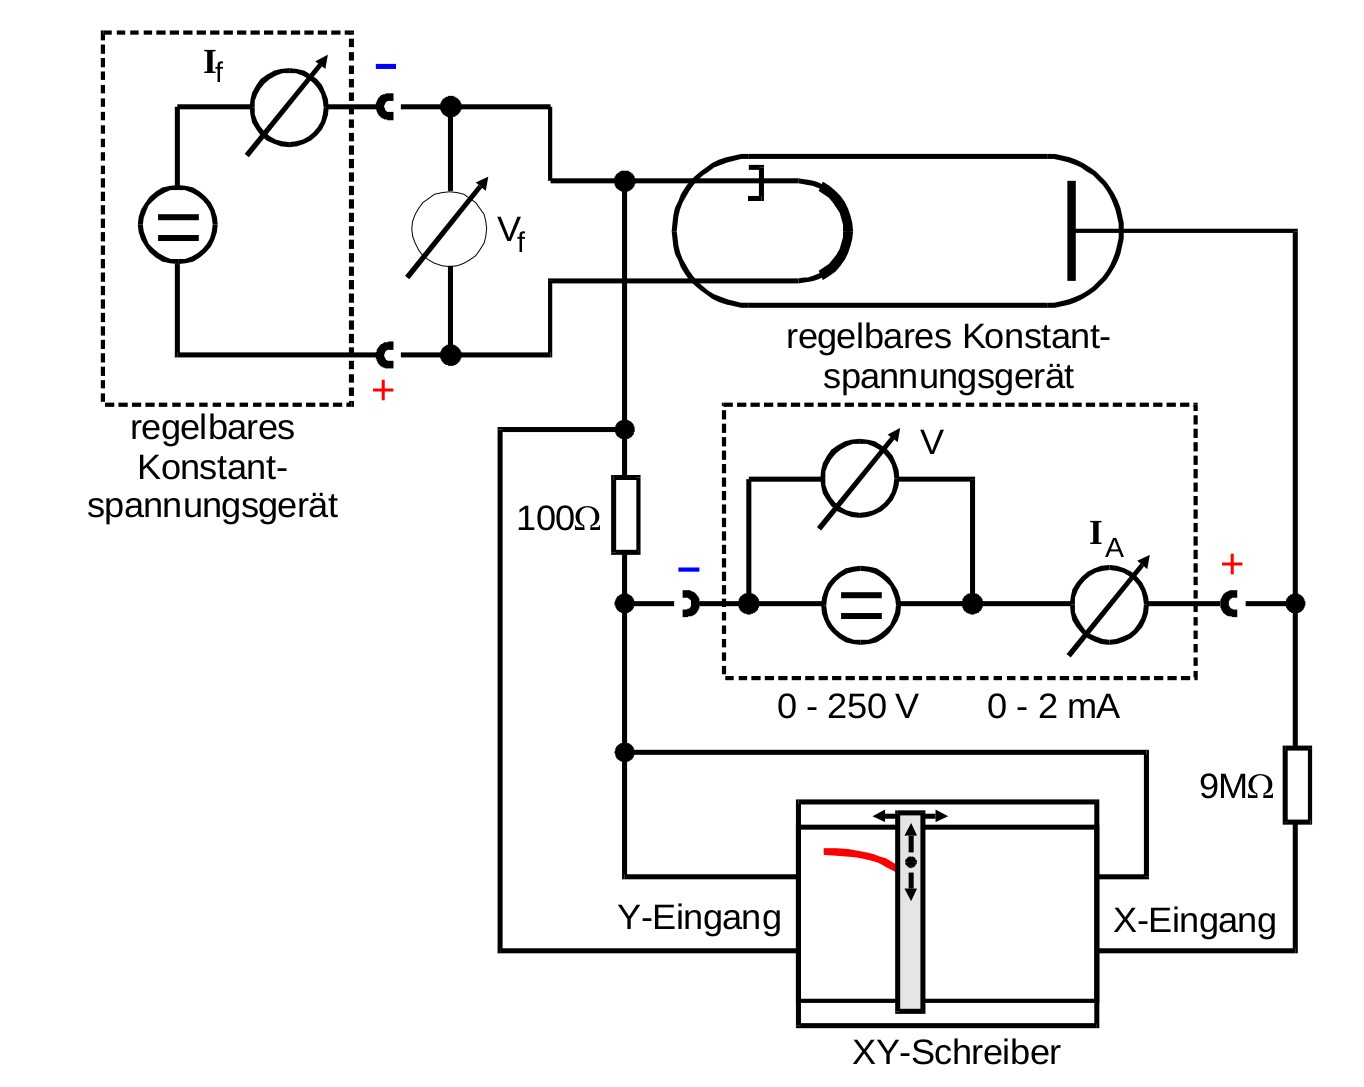
\includegraphics[scale=0.2]{content/Aufbau1.jpg}
  \caption{Messaufbau zur Bestimmung der Kennlinie [1].}
  \label{fig:aufbau1}
\end{figure}

\subsection{Ermittlung der Anlaufstromkurve}

Hierzu wird die Schaltung aus Abbildung \ref{fig:aufbau2} benutzt. Um den Anlaufstrom $I$ von 
der Größenordnung $\SI{1}{\nano\ampere}$ zu messen, wird ein empfindliches 
Nanoamperemeter mit eingebautem Verstärker benutzt. Wegen der geringen Ströme wird 
ein möglichst kurzes Kabel zwischen Anode und Eingangsbuchse HI verwendet. Durch 
den Innenwiderstand $R_\text{i}$ des Amperemeteres von $\SI{1}{\mega\ohm}$ liegt
zwischen Anode und Kathode eine andere Soannung $V$ an, als die vom 
Konstantsspannungsgerät angezeigte Spannung $U$. Die Heizspannung muss auf 
den Maximalwert gedreht werden, damit ein Strom gemessen werden kann. 
Der Strom wird in Abhängigkeit von der angelegten Diodenspannung abgelesen. 

\begin{figure}
  \centering
  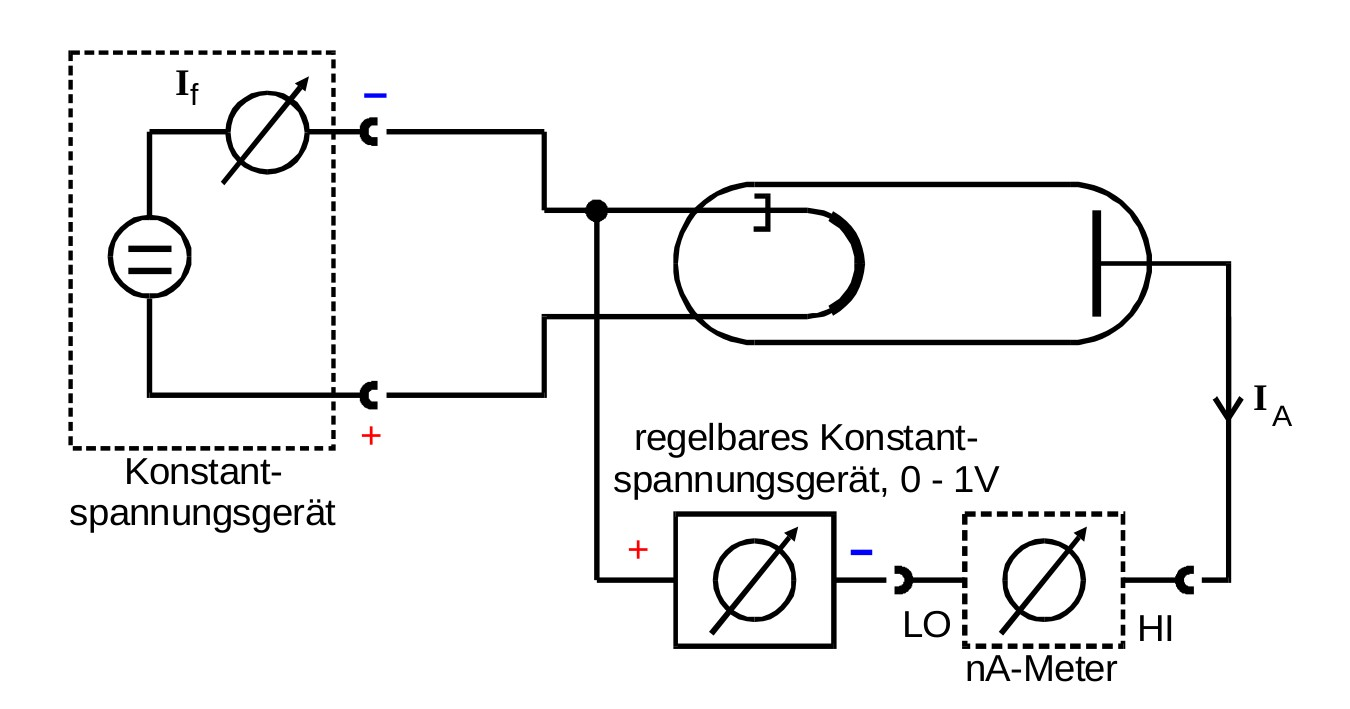
\includegraphics[scale=0.2]{content/Aufbau2.jpg}
  \caption{Schaltung zur Emittlung des Anlaufstroms [1].}
  \label{fig:aufbau2}
\end{figure}